\documentclass{report}
\usepackage{graphicx} % Required for inserting images
\usepackage[italian]{babel}
\usepackage{tikz}
\usepackage{hyperref}
\usepackage{amsmath}
\usepackage{xcolor}
\usepackage{float}
\usepackage{soul}
\usepackage{listings} % Per evidenziare il codice

\definecolor{lightgray}{rgb}{0.9,0.9,0.9} % Definizione colore sfondo
\definecolor{darkgreen}{rgb}{0.0, 0.5, 0.0}

\lstset{
    backgroundcolor=\color{lightgray}, % Sfondo grigio
    basicstyle=\ttfamily, % Font monospaziato
    % frame=single, % Bordo attorno al codice
    tabsize=4, % Dimensione tabulazione
    breaklines=true, % Permette di andare a capo automaticamente
    numbers = left,
    numberstyle=\small\color{gray}
}

\title{\huge\textbf{{Differential Privacy}}}
\date{Parte IV}
\begin{document}

\maketitle
\tableofcontents
\newpage

\chapter{Introduzione}
Introdotto nel 2006, ha avuto un'esplosione di utilizzo di questo concetto negli ultimi anni.

\noindent L'idea è la protezione dei dati, i dati sono privati e non basta che siano semplicemente anonimizzati.


\chapter{Basic Scenario}
\begin{figure}[H]
        \centering
        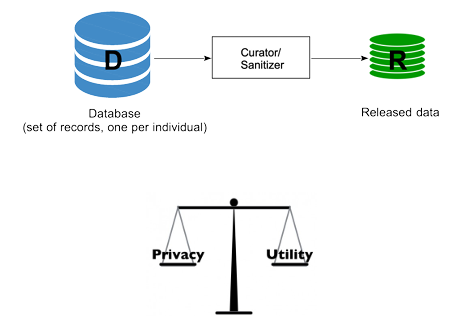
\includegraphics[width=0.6\linewidth]{images/basicScenario.png}
    \end{figure}

\begin{enumerate}
    \item \textbf{D:}Bisogna avere molti dati (se no D.P. non funziona bene), pensiamo di avere tanti record e ciascun record riguarda dati sensibili di individui.
    \item \textbf{Curator/Sanitizer:} è una parte fidata che può accedere in chiaro ai dati
    \item \textbf{R:} Dati rilasciati 
\end{enumerate}

\section{L'intuizione classica per la privacy}
Cosa vuol dire mantenere la privacy degli individui?
\begin{itemize}
    \item Ciò che viene rilasciato non dipende dai miei dati
    \item le informazioni apprese su un individuo dai risultati pubblicati R non sono più di quelle che possiamo apprendere su quell'individuo senza avere accesso a R.
\end{itemize}

\noindent \textbf{Problema:} Se gli individui non hanno impatto sui risultati allora i risultati non avrebbero utilità, serve equilibrio.

\section{Differential privacy– Intuition}
Quello che cerca di fare D.P. è che la presenza o l'assenza di un utente no cambi di molto il rischio di compromettere la sua privacy.
Chiaramente il rilascio di informazioni impone che un minimo cambiamento ci sia, però sia minimale.
Le inferenze che io posso fare su un individuo da un rilascio R deve essere lo stesos che io posso inferire utilizzando i dati di qualunque altro utente.
\begin{figure}[H]
        \centering
        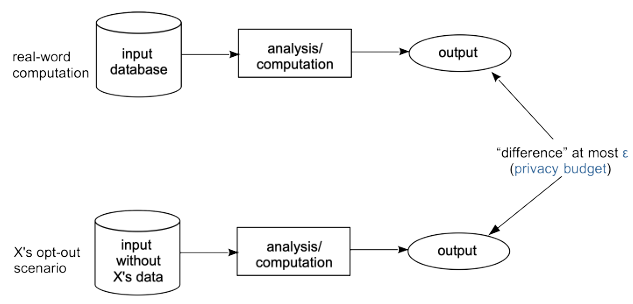
\includegraphics[width=0.6\linewidth]{images/intuition.png}
    \end{figure}

\noindent Più questo $\epsilon$ è piccolo più la differenza dei dati con, o senza, un determinato individuo è minimale.
Tutto questo viene fatto inniettando del rumore all'interno della mia computazione. Deve essere rumore casuale (NON deterministico)

\noindent Due principali complicazioni:
\begin{itemize}
    \item Capire quanto rumore inniettare
    \item Il risultato è sempre diverso poichè ogni volta viene inserita una quantità di rumore diversa (se viene posta la stessa domanda troppe volte si riesce a inferire il valore corretto, da questo nasce
    la necessità del \textbf{Privacy budget})
\end{itemize}










\end{document}